\subsection{Ingresos y egresos}

\subsubsection{Ingresos}

El modelo de ingresos contempla los planes de inversión de personas naturales y de empresas, las personas naturales y las empresas pueden usar el plan si registrarse pero sin muchos beneficios, las personas naturales pueden ingresar a un plan premium donde pueden recibir recomendaciones mucho mas personalizadas, las empresas pueden pagar por un plan mediano para acceder a estadísticas básicas en sus establecimientos o pagar extra para mostrar publicdad y obtener aún mas información sobre su empresa a ojos del turista.

  \vspace{2mm}
    \begin{minipage}{0.9\textwidth}
    \centering
    \captionof{table}[{Ingresos}]{Ingresos}
    \label{Ingresos}
    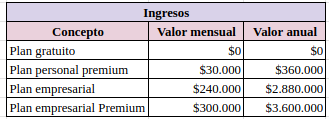
\includegraphics[width=0.9\textwidth]{Content/Images/AF/ingresos.png}
    \footnote{Nota. \textup{Fuente : Autores.}}
    \end{minipage}


\subsubsection{Egresos}
Durante el primer año, el equipo estará conformado por las dos personas que lideran el proyecto, quienes recibirán su remuneración conforme a las obligaciones legales y aportes parafiscales establecidos en Colombia. También se incluyen los costos asociados a la infraestructura virtual necesaria para operar. La tabla \ref{egresos} muestra un desglose detallado de estos gastos.

\vspace{2mm}
    \begin{minipage}{0.9\textwidth}
    \centering
    \captionof{table}[{Egresos}]{Egresos}
    \label{Ingresos}
    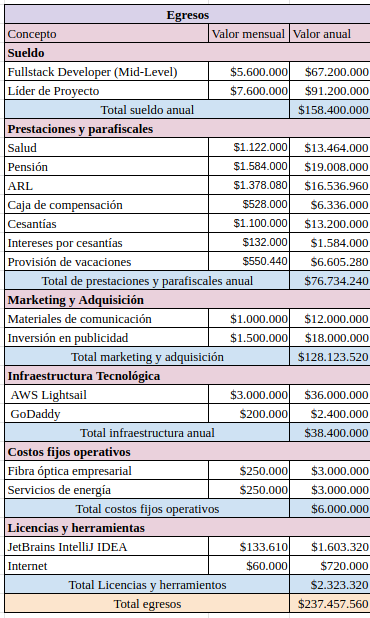
\includegraphics[width=0.9\textwidth]{Content/Images/AF/egresos.png}
    \footnote{Nota. \textup{Fuente : Autores.}}
    \end{minipage}